\documentclass[10pt, letterpaper]{article}

\usepackage[utf8]{inputenc}
\usepackage[spanish]{babel}
\usepackage{amsmath}
\usepackage{amsfonts}
\usepackage{amssymb}
\usepackage{graphicx}
\usepackage{epstopdf}
\usepackage{url}
\usepackage{booktabs}
\usepackage{caption}
\usepackage{float}
\usepackage{tikz}
\usepackage{subcaption}
\usetikzlibrary{calc}
\usepackage{titlesec}
\usepackage[left=2.2cm, right=2.2cm, top=2.0cm, bottom=2.0cm]{geometry}

\titlespacing*{\section}{0pt}{8pt}{3pt}
\titlespacing*{\subsection}{0pt}{6pt}{2pt}
\setlength{\parskip}{0pt}
\captionsetup{font=small, skip=3pt}

% Estilos del diagrama de bloques
\tikzset{
  bloque/.style={draw, rectangle, align=center, font=\scriptsize,
                 minimum height=0.80cm, inner sep=3pt},
  suma/.style={draw, circle, minimum size=0.58cm, inner sep=0pt,
               font=\footnotesize},
  senal/.style={->, thick, >=latex},
  etiqueta/.style={font=\scriptsize, inner sep=1.5pt}
}


\begin{document}
\begin{center}
    {\LARGE Proyecto --- Parte 2: Dinámica inversa, modelado y control de un \textit{drawing manipulator} de 2 GdL}
\end{center}
\textbf{Estudiantes: }
\begin{enumerate}
    \item José Elkin Estrada Morales - \url{estradam_jose@javeriana.edu.co}
    \item Juan David Rodríguez Franco  - \url{juandrodriguezf@javeriana.edu.co}
    \item David Santiago Mojica Lugo -
    \url{david-mojical@javeriana.edu.co}
\end{enumerate}

\section{Métodos y Desarrollos}

\subsection{Modelo de dinámica inversa}
% P8: pendiente

\subsection{Modelado de motores y sensores}

El S3003 es un servo integrado: incluye motor, reductora, potenciómetro y
controlador analógico. El lazo de posición ya viene cerrado y el servo solo
recibe PWM; por eso, para simulación se adopta un motor DC equivalente de primer
orden referido al eje de salida, calibrado con el datasheet \cite{futaba}. En la
parte experimental se usa el S3003 tal como se compró.

El modelo se implementó en MATLAB/Simulink con una instancia por grado de
libertad: \texttt{Joint1} y \texttt{Joint2} en \texttt{motor\_2gdl.slx}. Cada
instancia incluye la planta DC y los sensores de posición, corriente y velocidad
necesarios para el control de bajo nivel de su articulación. La figura
\ref{fig:diagrama} presenta el diagrama de una instancia (\texttt{Joint1}); el
modelo completo contiene dos instancias idénticas, \texttt{Joint1} y
\texttt{Joint2}, una por grado de libertad. Los parámetros se ajustaron con el
datasheet del S3003. No se usó Simscape Electrical porque no está licenciado; se
emplearon bloques base de Simulink.

\begin{figure}[H]
    \centering
    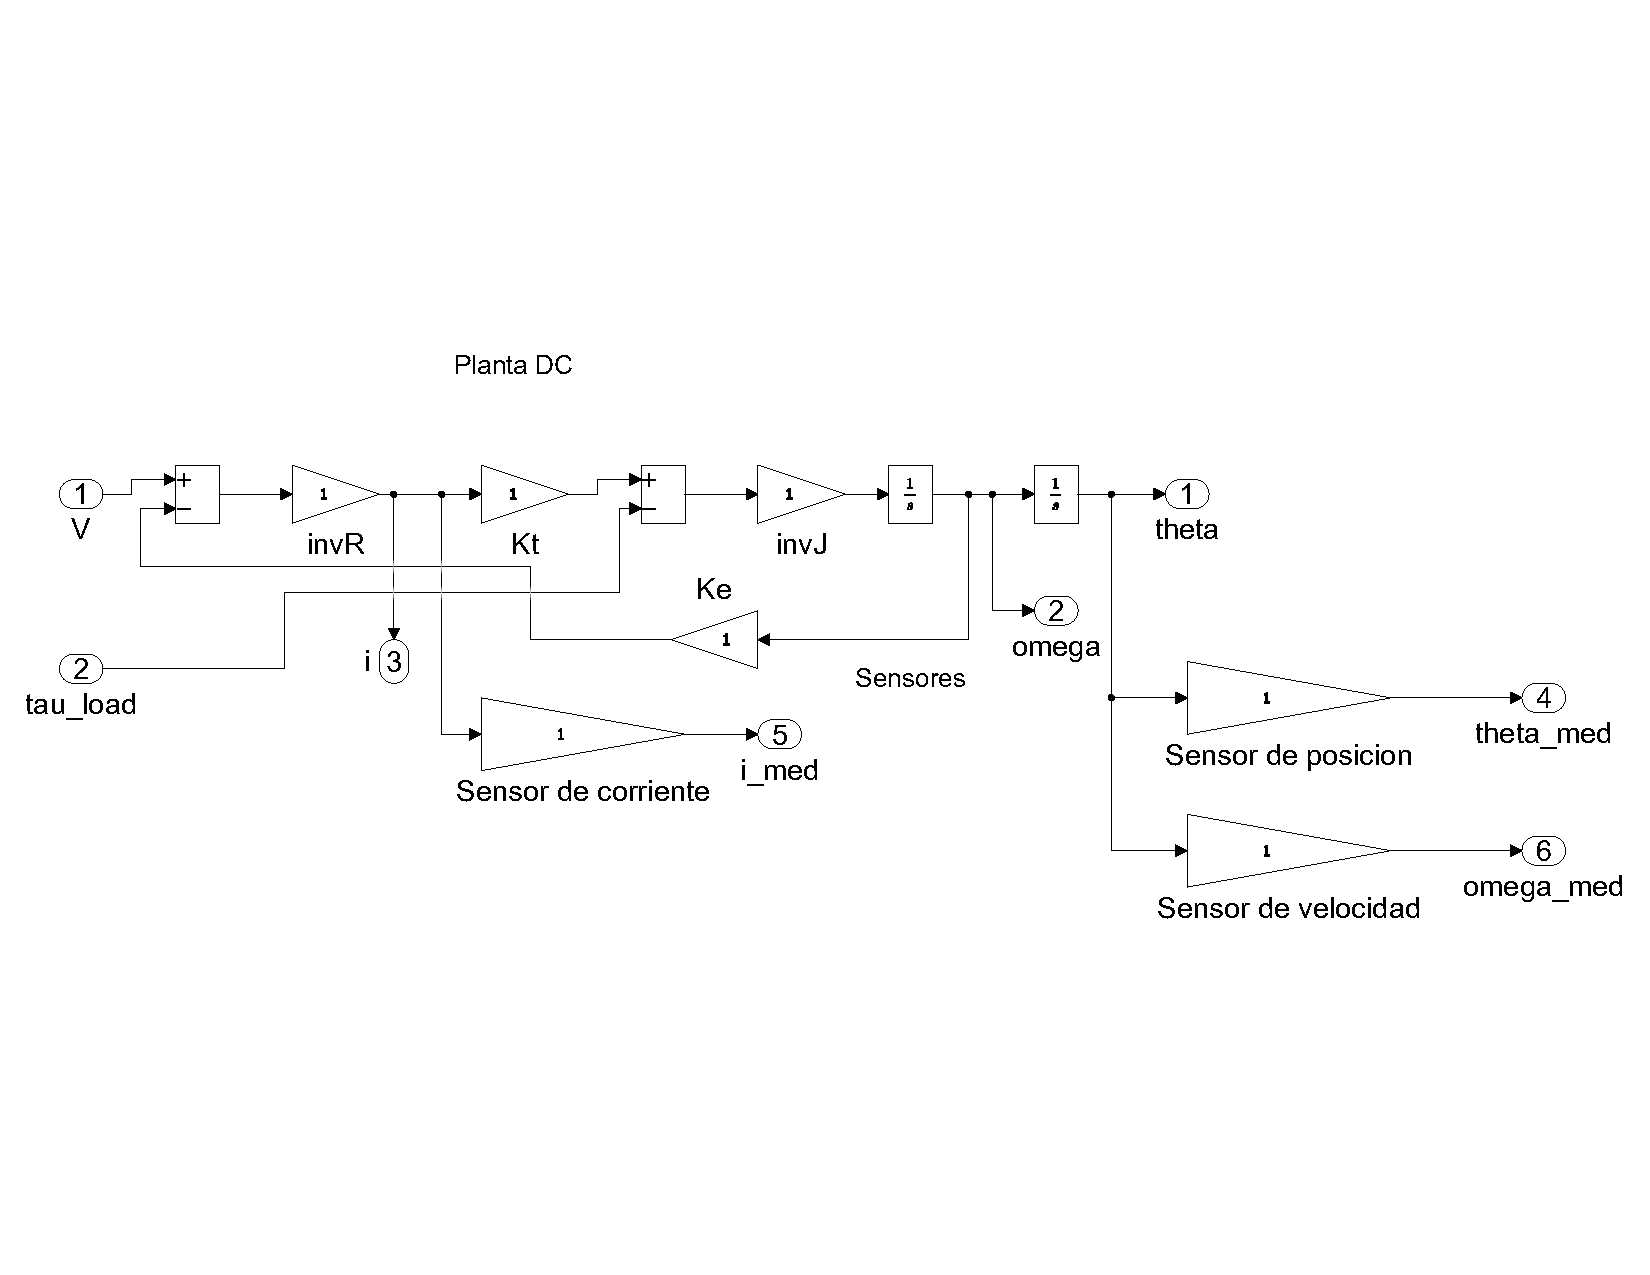
\includegraphics[width=0.95\linewidth,trim=11.85 170.79 12.69 169.76,clip]{figuras/motor_diagrama_sim.pdf}
    \caption{Diagrama de bloques de una instancia (\texttt{Joint1}) del modelo de motor y sensores (P10). El modelo completo contiene dos instancias idénticas, una por GdL.}
    \label{fig:diagrama}
\end{figure}

El modelo resuelve las ecuaciones
\begin{align}
    i &= \frac{V - K_e\omega}{R}, \label{eq:corriente}\\
    J\dot{\omega} &= K_t i - \tau_{load}, \label{eq:mecanica}\\
    \dot{\theta} &= \omega, \label{eq:cinematica}
\end{align}
donde $V$ es la tensión de entrada, $i$ la corriente, $\omega$ la velocidad y
$\theta$ la posición del eje de salida. La inductancia $L$ y el amortiguamiento
$B$ se desprecian para obtener el modelo de primer orden; $J$ se estima a partir
de un valor típico de servo pequeño. Los parámetros se resumen en la tabla
\ref{tab:parametros}.

\begin{table}[H]
    \centering
    \caption{Parámetros del motor equivalente.}
    \label{tab:parametros}
    \small
    \begin{tabular}{lcc}
        \toprule
        Parámetro & Valor & Fuente \\
        \midrule
        $K_e = K_t$ & $1{,}0886$ V$\cdot$s/rad $=$ N$\cdot$m/A & Datasheet \\
        $R$ & $16{,}245$ $\Omega$ & Datasheet \\
        $J$ & $3\times10^{-4}$ kg$\cdot$m$^2$ & Estimada \\
        $L$ & $0$ & Despreciada \\
        $B$ & $0$ & Despreciada \\
        $V_{max}$ & $6$ V & Datasheet \\
        $\omega_{nl}$ & $5{,}5116$ rad/s & Datasheet \\
        $\tau_{stall}$ & $0{,}4021$ N$\cdot$m & Datasheet \\
        $i_{stall}$ & $0{,}3693$ A & Derivada \\
        $K = 1/K_e$ & $0{,}9186$ rad/s/V & Derivada \\
        $\tau_m = JR/(K_tK_e)$ & $4{,}11$ ms & Derivada \\
        \bottomrule
    \end{tabular}
\end{table}

Los sensores se modelan de forma genérica, porque el S3003 no expone el
potenciómetro ni la corriente del motor. La tabla \ref{tab:sensores} resume sus
características.

\begin{table}[H]
    \centering
    \caption{Sensores modelados para el control de bajo nivel de cada GdL.}
    \label{tab:sensores}
    \small
    \begin{tabular}{lcc}
        \toprule
        Sensor & Modelo & Parámetros \\
        \midrule
        Posición  & Cuantización $+$ ruido $+$ saturación & $\pm90^\circ$; $0{,}5^\circ$; $0{,}05^\circ$ \\
        Corriente & Filtro $+$ ruido $+$ saturación & $\pm1$ A; $2$ mA; $1000$ Hz \\
        Velocidad & Derivada filtrada & $20$ Hz \\
        \bottomrule
    \end{tabular}
\end{table}

El periodo de muestreo es $T_s=0{,}01$~s. La carga mecánica se incluye como
series de tiempo \texttt{tau1} y \texttt{tau2}, calculadas con
\texttt{carga\_mecanica.m}; el par máximo es $0{,}177$~mN$\cdot$m y su efecto en
la velocidad es $0{,}0013$~rad/s ($0{,}024\%$).

\paragraph{Verificación del modelo.}
La tabla \ref{tab:verificacion} resume la verificación del modelo de P10 contra
el datasheet.

\begin{table}[H]
    \centering
    \caption{Verificación del modelo de P10.}
    \label{tab:verificacion}
    \small
    \begin{tabular}{lcc}
        \toprule
        Prueba & Esperado & Obtenido \\
        \midrule
        $\omega_{nl}$ a 6 V & $5{,}5116$ rad/s & $5{,}5116$ rad/s \\
        $\omega_{nl}$ a 3 V & $2{,}7558$ rad/s & $2{,}7558$ rad/s \\
        $\tau_m$ & $4{,}11$ ms & $4{,}3$ ms \\
        $i_{stall}$ & $0{,}3693$ A & $0{,}3693$ A \\
        $\tau_{stall}$ & $0{,}4021$ N$\cdot$m & $0{,}4021$ N$\cdot$m \\
        $\Delta\omega$ con carga mecánica & $0$ & $0{,}0013$ rad/s \\
        \bottomrule
    \end{tabular}
\end{table}

El modelo reproduce la velocidad sin carga y el par de bloqueo; la carga
mecánica es despreciable. La posición medida tiene un error máximo de
$0{,}28^\circ$ y la corriente un error máximo de $0{,}271$~A en el escalón
(RMS $0{,}0168$~A). La velocidad derivada es ruidosa (RMS $0{,}754$~rad/s). Las
figuras \ref{fig:escalon} y \ref{fig:sensores} muestran las respuestas y los
sensores.

\begin{figure}[H]
    \centering
    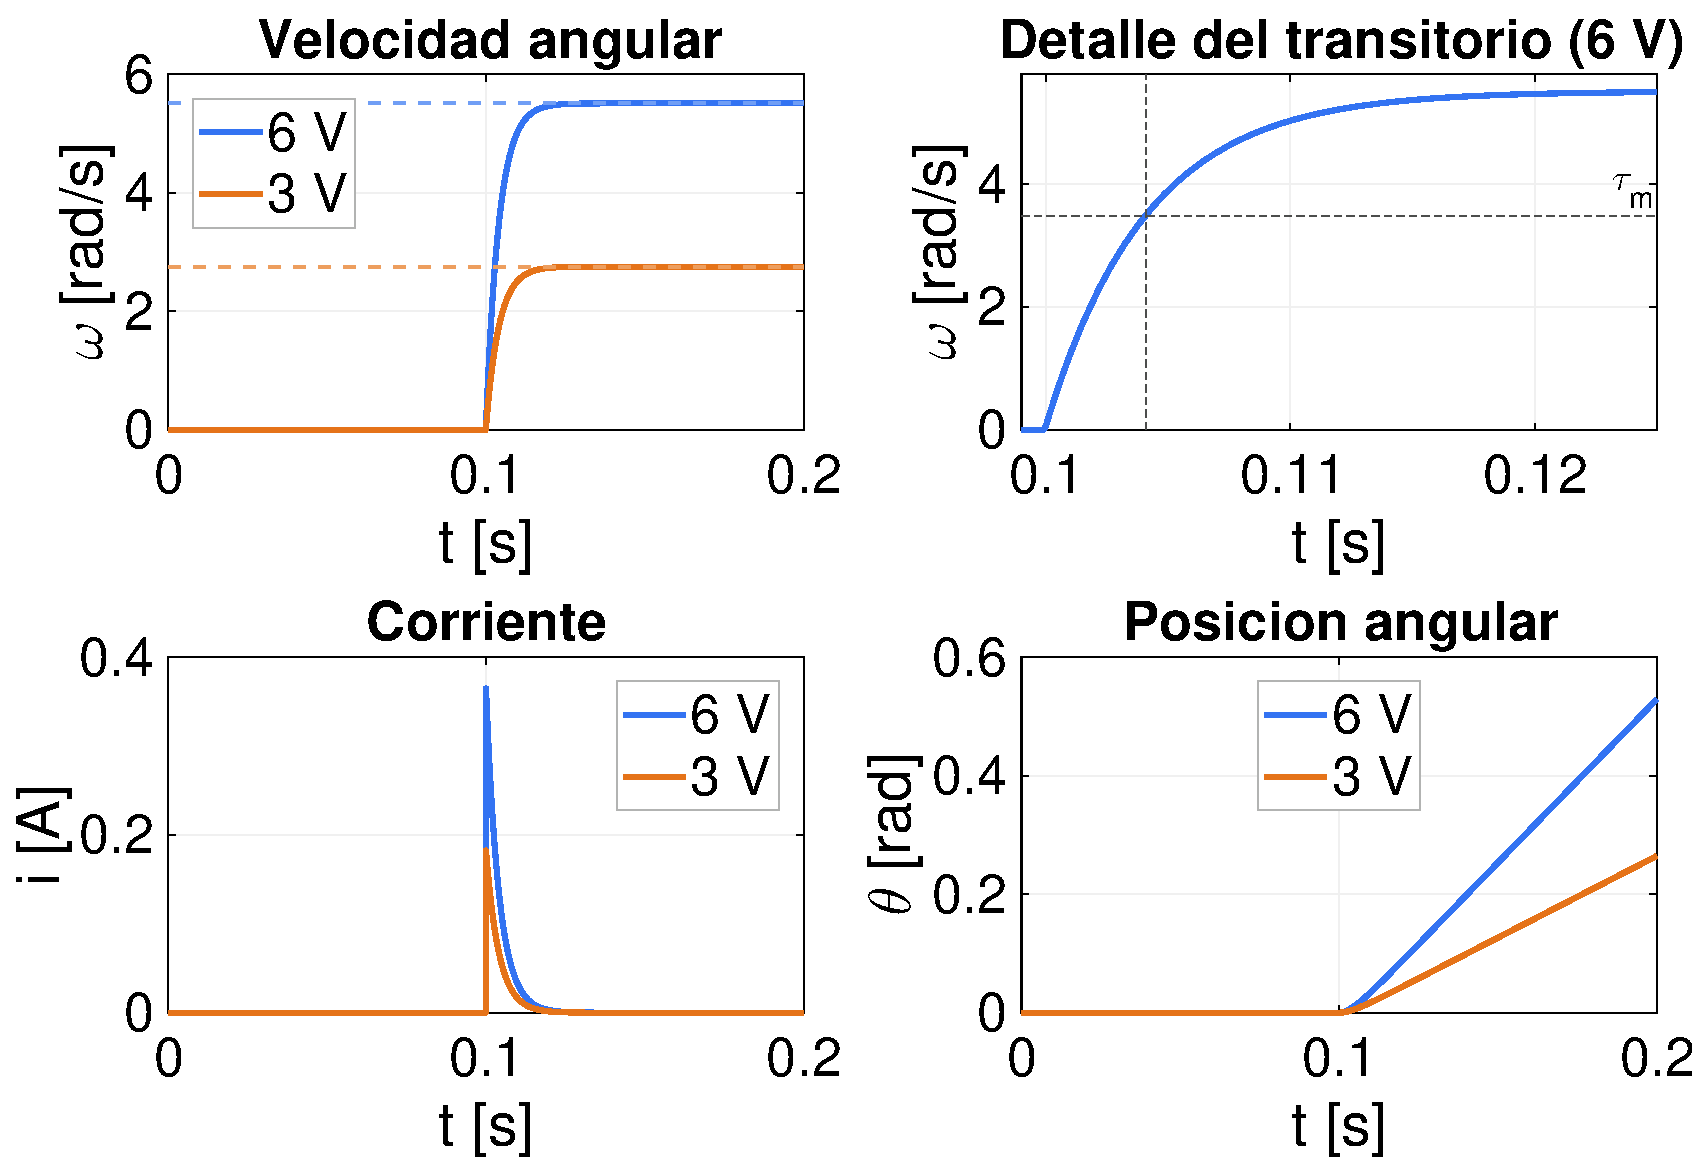
\includegraphics[width=0.90\linewidth]{figuras/motor_escalon.eps}
    \caption{Respuesta del modelo a escalones de 6 V y 3 V.}
    \label{fig:escalon}
\end{figure}

\begin{figure}[H]
    \centering
    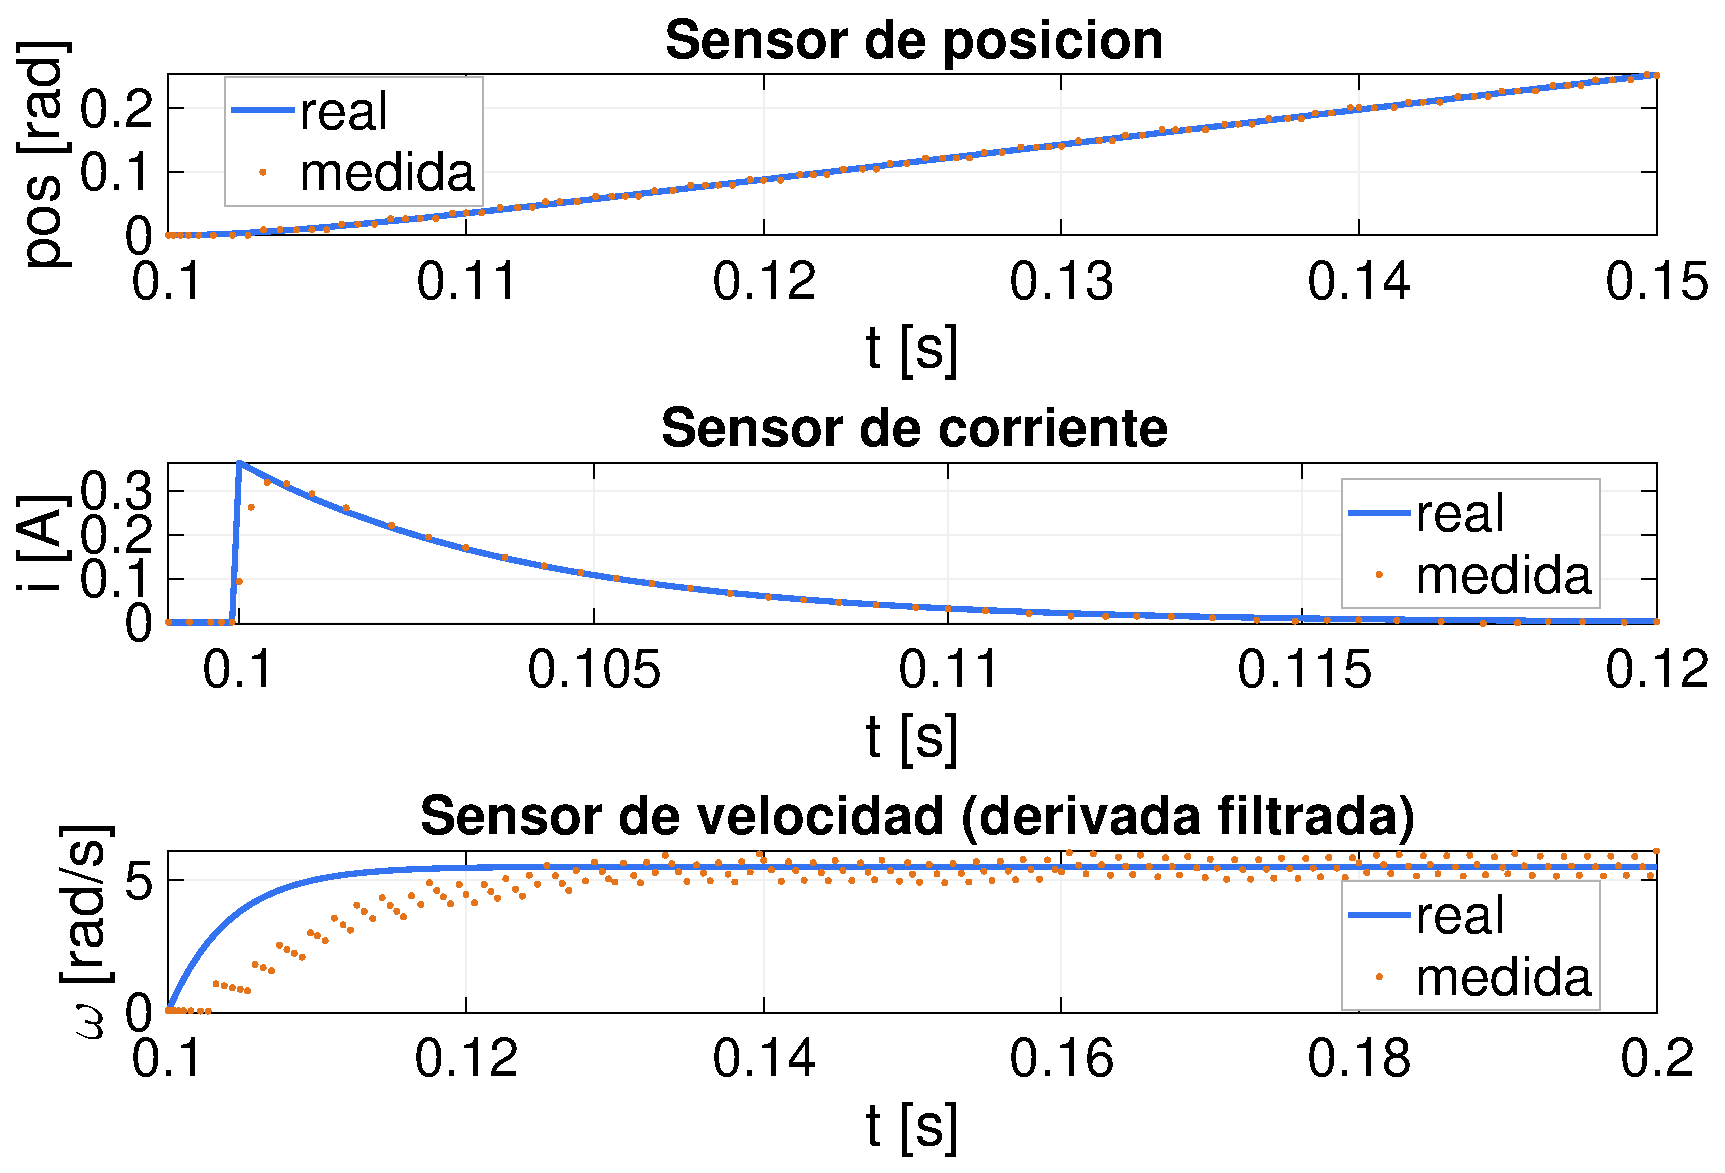
\includegraphics[width=0.70\linewidth]{figuras/motor_sensores.eps}
    \caption{Señales reales y medidas de los sensores de posición, corriente y velocidad.}
    \label{fig:sensores}
\end{figure}

\subsection{Control de bajo nivel}
% P11: pendiente

\section{Resultados}

\subsection{Resultados de dinámica inversa}
% P8: pendiente

\subsection{Simulación de control}
% P11: pendiente

\section{Conclusiones}
% Pendiente

\bibliographystyle{ieeetr} % Define el estilo de formato (puedes cambiarlo por plain, unsrt, etc.)
\bibliography{referencias} % Llama a tu archivo .bib (no incluyas la extensión .bib aquí)


\end{document}
